\section{Jeu de la somme magique}

\subsection{Représentation sous forme de morpion}
Ce jeu, comme expliqué dans les transparents présentés en cours,
consiste à choisir, à tour de rôle, $n$ nombres parmi $n^2$ afin que
leur somme soit égale à $\frac{n(n^2+1)}{2}$.

Une représentation possible de ce jeu est le carré magique: les
joueurs doivent choisir, l'un après l'autre une case dans un carré
magique, leur but étant de contrôler une ligne, une colonne ou une
diagonale entière du carré magique; alors, les nombres qu'ils auront
choisis totaliseront le score voulu. De même, ce problème correspond exactement
au jeu du morpion, étendu à des grilles $n \times n$.

Ainsi, une des stratégies possibles pour un joueur du jeu de la somme
magique est de construire un carré magique, et de représenter les
nombres choisis par l'adversaire par un rond dans la case
correspondante. Afin de choisir un nombre, il suffit d'appliquer la
stratégie de morpion de son choix sur le carré magique, et de
jouer le nombre correspondant.

Le choix du carré magique n'importe pas. En effet, dans un carré
magique sont présentes toutes les possibilités de combinaison de
nombres pour obtenir la somme voulue. Par conséquent, peu importe le
carré magique d'ordre $n$ que l'on choisit, les représentations sous forme de
morpion seront toutes équivalentes.

Le morpion étant un jeu où l'on essaie de minimiser la perte maximum,
on peut s'intéresser à l'algorithme du minmax, pour déterminer une
stratégie non-perdante.

\subsection{Algorithme du minmax appliqué au jeu du morpion}
L'algorithme du minmax consiste à évaluer toutes les positions de jeu
atteignables depuis la position courante, sur une certaine profondeur
(autrement dit, un certain nombre de tours de jeu), et à jouer de
manière à atteindre la position la plus avantageuse, en supposant que
l'adversaire joue toujours le meilleur coup pour lui-même (ce coup
étant évalué avec notre propre fonction d'évaluation, qui n'est pas
forcément la même que celle de l'adversaire).

Par conséquent, afin d'implémenter l'algorithme du minmax, il faut
commencer par déterminer une fonction d'évaluation.

\subsubsection{Fonction d'évaluation}
La fonction d'évaluation que nous avons choisie est très simple: une
ligne, colonne ou diagonale (que nous appelleront désormais simplement
``ligne'') complétée avec notre symbole (ce qui signifie qu'on a
gagné) vaut $+\infty$; si, au contraire, l'adversaire a complété une
ligne, alors cette ligne vaut $-\infty$. Une ligne contenant
uniquement notre symbole rapporte le nombre d'occurrences de notre
symbole dans cette ligne ; à l'inverse, une ligne contenant uniquement
le symbole de l'adversaire rapportera négativement le nombre
d'occurrences de ce symbole dans cette ligne.
Toutes les autres lignes ne rapportent aucun point.
Ainsi, l'évaluation d'une position de jeu est la somme des points
rapportés par chacune de ses lignes, colonnes et diagonales.

\subsubsection{Minmax}
L'algorithme du minmax va construire (implicitement) l'arbre des coups
possibles à partir de la position courante.
L'évaluation d'un nœud de cet arbre sera:
\begin{itemize}
  \item si c'est à notre tour de jouer, le maximum de l'évaluation de nos fils;
  \item si c'est à l'adversaire de jouer, le minimum de l'évaluation
    de ses fils (i.e.\ on suppose que l'adversaire joue le meilleur
    coup à sa disposition, selon la fonction d'évaluation du joueur courant).
\end{itemize}

L'évaluation d'une feuille de l'arbre se fera par la fonction
d'évaluation définie précédemment.

Ainsi, l'algorithme se dirigera naturellement vers la position la plus
avantageuse pour lui.

\subsection{Élagage alpha-bêta}
L'élagage alpha-bêta permet de réduire le nombre de nœuds à parcourir durant
l'algorithme du minmax.

Cette algorithme arrête le parcours des fils d'un nœud quand il se rend
compte qu'il ne pourra pas faire mieux.

Dans l'exemple suivant, où les nœuds en bleus sont ceux où l'on doit prendre
le minimum, et ceux en gris le maximum :
\begin{center}
  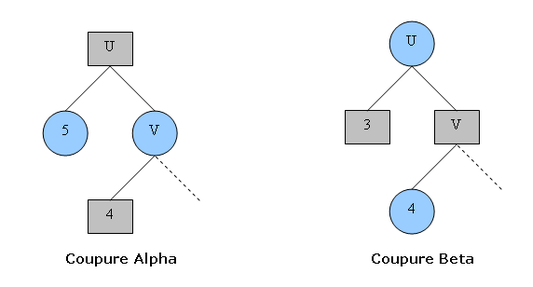
\includegraphics[width=300px]{coupures_alpha-beta.png}
\end{center}

On se rend bien compte qu'on n'a pas besoin de parcourir les nœuds suivant,
car on prend le maximum des minimums, ou l'inverse.

Par exemple, pour la coupure alpha : si on trouve des fils de $V$ plus petit
que $4$, on va prendre le maximum, donc c'est $4$ qui sera utilisé, et si on
trouve plus grand ou égal à $5$, on devra prendre le minimum au niveau de $V$,
donc on prendra $5$ dans tous les cas.

Au final, cette amélioration permet de gagner un temps considérable.

\subsection{Résultats}
\subsubsection{Meilleure stratégie}
Nous avons fait s'affronter différentes stratégies les unes contre les
autres, afin de voir laquelle était la meilleure, sur différentes
tailles de plateaux. Les stratégies que nous avons fait s'affronter
étaient:
\begin{itemize}
  \item la stratégie aléatoire,
  \item la stratégie qui prend toujours la première case disponible,
  \item les stratégies utilisant le minmax à différentes profondeurs,
    entre 2 et 10,
  \item les stratégies utilisant le minmax et l'élagage alpha-bêta à
    différentes profondeurs, entre 2 et 10.
\end{itemize}
Les résultats ne sont guère surprenants: toutes les stratégies
parviennent au match nul, à l'exception des stratégies aléatoires et
premier\_dispo, qui perdent systématiquement contre un minmax de
profondeur supérieure à 2.

\subsubsection{Performances}
Du point de vue du temps d'exécution, toutefois, l'algorithme avec
élagage est beaucoup plus rapide qu'un minmax simple, alors qu'il
retourne le même résultat.
Malheureusement, nous n'avons pas pu tester nos algorithmes sur des
plateaux de grande taille: en effet, à partir de la taille 4, un
minmax avec élagage de profondeur 10 met en moyenne 5 secondes pour
décider de son coup, et peut aller jusqu'à 40s!

Il est également intéressant de noter, bien que ceci n'ait rien à voir
à notre projet, que le passage du langage Python au langage C a permis
de diviser le temps d'exécution des tests par 60 pour des stratégies
sans élagage.
